%% set up
\documentclass[11pt]{article}

%% packages
\usepackage[margin=1in]{geometry} % Required to make the margins smaller to fit
% more content on each page 
\usepackage[utf8]{inputenc}
\usepackage{enumitem}
\usepackage{graphicx}
\usepackage{listings}
\usepackage{xcolor}
\usepackage{amsfonts}
\usepackage{mathtools}
\usepackage{booktabs}
\usepackage{pdflscape}
\usepackage{longtable}
\usepackage{amsmath}
\usepackage{pdflscape}
\usepackage{lmodern,textcomp} % for euro symbol

\setlist{itemsep=1pt} % This controls spacing between items in the lists
\setlength\parindent{0pt} % Removes all indentation from paragraphs

\title{Figures and Tables for 'Using Joint Species Distribution models to
	inform mixed fishery management'}
\author{Paul J. Dolder, James T Thorson, Cóilín Minto}
%%%%%%%%%%%%%%%%%%%%%%%%%%%%%%%%%%%%%%%%%%%%%
%%%%%%%%%%%%%%%%%%%%%%%%%%%%%%%%%%%%%%%%%%%%%
\begin{document}
\maketitle

\tableofcontents

\listoffigures

\listoftables

\newpage

To be used in methods, to show spatial assignment of static covariates:

\begin{figure}[!ht]
	\center
	\includegraphics[width = 0.8\linewidth]{../../plots/HabitatCovariatesPoly}
	\label{fig:HabCov}
	\caption{Substrate type and depth associated with each of the knots
		used to estimate species density}
\end{figure}


\newpage

Survey catchability estimates, 
Key points:

\begin{itemize}
	\item In keeping with expectation, the survey catchability estimates
		are generally higher for those species-gear combinations that
		are considered more efficient at catching a particular species
		type. E.g. the otter trawl surveys (THA2, CEXP, Q4SWIBTS and
		WCGFS) estimates are more similar to each other and have
		positive coefficients relative to the beam trawl surveys
		(Carlhelmar, Q1SWBeam and NWGFS) for the roundfish species and
		vice versa for the flatfish species.
	\item 2 species-gear combinations (carlhelmar juvenile cod and
		budegassa) were not estimated and instead fixed. 
\end{itemize}

\begin{figure}[!ht]
	\center
	\includegraphics[width = 0.9\linewidth]{../../results/2017-04-08_M2/QEstimatesALL}
	\label{fig:Q_inline}
	\caption[Gear catchability estimates]{Estimates of gear catchability
		covariates for each species.  Each parameter is estimated
		relative to the Celtic Explorer ('CEXP'). lambdak\_1 =
		Encounter probability, lambdak\_2 = Effect on positive catch
		rates. Red triangles indicate fixed parameters for Carlhelmar
		survey for cod\_juv and bud\_juv}
\end{figure}

\newpage

\begin{itemize}
	\item Within species correlations (among size classes) are strong, for
		all species. 
	\item Spatial encounter correlations are very strong for similar
		species types (i.e. gadoids: cod, haddock, whiting and hake;
		flatfish: plaice, sole....also with whiting, haddock)
	\item Spatio temporal encounter correlations are broadly similar,
		though weaker and tend also to co-occur among more species,
		implying that some species are found together some but not all
		the time.
	\item  Spatial catch rates tend to correlate within a species class and
		also among some groups (e.g. cod with budegassa, haddock,
		whiting and hake; haddock strongly with whiting)
	\item Spatio temporal catch rates again are broadly similar, yet found
		among more species groups (e.g. also cod with plaice)
		suggesting that some species are found together, but not all
		the time.

\end{itemize}

\begin{figure}[!ht]
	\includegraphics[width = \linewidth]{../../results/2017-04-08_M2/Spatio-temporal_covariances--Analytic}
	\label{fig:Corr}
	\caption{Inter-species correlations}
\end{figure}

\newpage

Key points:
\begin{itemize}
	\item Factor analysis shows common trend for encounter probability
		based on spatial gradient from nearshore to offshore (seen in
		Figure 4, Figure 5 factor maps, omega). There is no clear species
		grouping (Figure 14, PCA / factor loadings). 
	\item This could mean that the probability of encountering a species
		can be consistently described through a combination of
		spatially determined factors (linked to depth, distance from
		shore etc.. (?? though habitat covariates appear uninformative) 
	\item Conversely, the positive catch rates spatio-temporal effect is
		better described through linkage among species groups (Figure
		6, PCA / factor loadings). The first two factors separate among
		the key species groups (roundfish, flatfish and deep water
		species). However, there is not as clear a spatial pattern
		(Figure 15, factor maps, epsilon).
	\item 	This could be because that catch rates are much more variable
		in time, not linked to a spatial pattern but consistent among
		groups of species (can this be an environmental driver???).
		Would be good to include a temporally changing environmental
		predictor (e.g. temperature - we could do this...) 
	\item  Overall, it appears encounter probability for each species
		remains stable over time (and predictable) based on spatial
		factors.  Positive catch rates are much, much more dynamic from
		year to year, though appears some common linkage among species
		groups.
\end{itemize}


\begin{figure}[!ht]
	\includegraphics[width	=\linewidth]{../../results/2017-04-08_M2/Factor_maps--Omega1}
	\label{fig:FactMap1}
	\caption{Factor plot for spatial encounter probability : maybe first 2
	-3 is enough ?}
\end{figure}

\begin{figure}[!ht]
	\includegraphics[width	=\linewidth]{../../results/2017-04-08_M2/Factor_maps--Omega2}
	\label{fig:FactMap2}
	\caption{Factor plot for spatial positive catch rates: maybe first 2-3
	is enough}
\end{figure}

\begin{figure}[!ht]
	\includegraphics[width 	=\linewidth]{../../results/2017-04-08_M2/PCAstyle_Plots_Spatiotemporal}
	\label{fig:PCA2}
	\caption{PCA style plots for spatio-temporal encounter probability and
		positive catch rates. N.B. It would be quite cool to do these
		points as images of the fish, would show clustering of
		flatfish, gadoid etc..}
\end{figure}

\newpage

Specific spatial pattens for density of cod, haddock and whiting (Figure 7):

\begin{itemize}
	\item Cod / haddock relative distribution shows weak separation north to
	south, with more cod north and more haddock south.
	\item cod and whiting relative distributions show weak separation east
		and west. With more cod west and more whiting east.
	\item haddock and whiting show weak separation east and west, with
		more haddock west and more whiting east.
\end{itemize}

\begin{figure}[!ht]
	\centering
	\includegraphics[width	= \linewidth]{../../plots/Density_Differences}
	\label{fig:DensityDiff}
	\caption{Plot of difference between normalised density estimates in
		2015 for selected species. The proportion of each species in
		each area are calculated, and the difference for each area is
		[spp1 - spp2]. The scale ranges from -6 \% to + 2 \%. Blue indicates
		more of species 1 (LHS),red more of species 2 (RHS).  White
		indicates no difference}
\end{figure}


%%%%%%%%%%%%%%%%%%%%%%%%%%%%%%%%%%%%%%%%%%%%%%%%%%%%%
%% Tables

\newpage

\textbf{Tables}

\begin{table}[!ht]
	\caption{List of species codes and names}
	\center
	\begin{tabular}{ p{3cm} p{4cm} p{5cm} }
		\hline
		Species code & Common name              & Species \\
		\hline
		juv          & Juvenile                 & \\
		adu          & Adult                    & \\
		\hline
		bud          & Black bellied anglerfish & \textit{Lophius budgessa} \\
		cod          & Atlantic cod             & \textit{Gadus morhua} \\
		had          & Atlatic haddock          & \textit{Melanogrammus aeglefinus} \\
		hke          & Atlantic hake            & \textit{Merluccius merluccius} \\
		meg          & Megrim                   & \textit{Lepidorhombus whiffiagonis} \\
		pisc         & White bellied anglerfish & \textit{Lophius piscatorius}	\\
		ple          & European Plaice          & \textit{Pleuronectes platessa} \\
		sol          & Common sole              & \textit{Solea solea} \\
		whg          & Atlantic whiting         & \textit{Merlangius merlangus} \\
		\hline
	\end{tabular}
\end{table}

\newpage

\begin{table}[!ht]
	\caption{List of survey codes, names and brief description}
	\center
	\begin{tabular}{ p{3cm} p{4cm} p{4cm} p{2cm} }
		\hline
		Survey code    & Name 	& Gear & Temporal extent \\
		\hline
		CEXP           & Celtic Explorer (IE)   & Otter trawl & 2003 - 2015 \\
		CARLHELMAR     & Carlhelmar (UK)	& Commercial beam trawl & 1989 - 2013 \\
		NWGFS          & North West groundfish survey (UK) & Beam trawl & 1988 - 2015 \\
		Q1SWBEAM       & Quarter 1 south-west beam trawl survey (UK) 	& beam trawl & 2006 - 2015 \\
		Q4SWIBTS       & Quarter 4 south-west international bottom trawl survey (UK) & Otter trawl & 2003 - 2010 \\
		THA2           & EVHOE survey on Thalasa (FR) & Otter trawl & 1997 - 2015 \\
		WCGFS          & Wstern channel groundfish survey (UK) & Otter
		trawl (Portugese high headline) & 1982 - 2004 \\
		\hline
	\end{tabular}
\end{table}


%%%%%%%%%%%%%%%%%%%%%%%%%%%%%%%%%%%%%%%%%%%%%%%%%%%%%%%%%%%%%%%%%%%%%%%%%%%%%%%%%%%%%%%%%%%%

\newpage

\textbf{Supplementary}

Some of the other plots which were quite informative.

\begin{figure}[!ht]
	\includegraphics[width = \linewidth]{../../results/2017-04-08_M2/QEstimatesGridEnc}
	\label{fig:Q_square1}
	\caption{as per Figure 2 but only showing lambdak\_1 }
\end{figure}

\begin{figure}[!ht]
	\includegraphics[width = \linewidth]{../../results/2017-04-08_M2/QEstimatesGridPos}
	\label{fig:Q_square2}
	\caption{as per Figure 2 but only showing lambdak\_2}

\end{figure}

%%%% Factor loadings 

\begin{figure}[!ht]
	\includegraphics[width =\linewidth]{../../results/2017-04-08_M2/Factor_loadings--Omega1}
	\label{fig:Fact1}
	\caption{Factor loadings - Omega 1, Spatial encounter}
\end{figure}

\begin{figure}[!ht]
	\includegraphics[width =\linewidth]{../../results/2017-04-08_M2/Factor_loadings--Omega2}
	\label{fig:Fact2}
	\caption{Factor loadings - Omega 2, Spatial catch rates}
\end{figure}

\begin{figure}[!ht]
	\includegraphics[width =\linewidth]{../../results/2017-04-08_M2/Factor_loadings--Epsilon1}
	\label{fig:Fact3}
	\caption{Factor loadings - Epsilon 1, Spatio-temporal encounter probability}
\end{figure}

\begin{figure}[!ht]
	\includegraphics[width =\linewidth]{../../results/2017-04-08_M2/Factor_loadings--Epsilon2}
	\label{fig:Fact4}
	\caption{Factor loadings - Epsilon 2, Spatio-temporal catch rates}
\end{figure}

\begin{figure}[!ht]
	\includegraphics[width 	=\linewidth]{../../results/2017-04-08_M2/PCAstyle_Plots_Spatial}
	\label{fig:PCA1}
	\caption{PCA style plots for spatial (Omega) encounter probability and positive catch rates}
\end{figure}

\begin{figure}[!ht]
	\includegraphics[width =\linewidth]{../../results/2017-04-08_M2/Factor_maps--Epsilon1}
	\label{fig:FactMap3}
	\caption{Spatial factor loading map - Epsilon 1, spatio-temporal encounter probability}
\end{figure}

\begin{figure}[!ht]
	\includegraphics[width	=\linewidth]{../../results/2017-04-08_M2/Factor_maps--Epsilon2}
	\label{fig:FactMap4}
	\caption{Spatial factor loading map - Epsilon 2, spatio-temporal positive catch rates}
\end{figure}

\begin{figure}[!ht]
	\center
	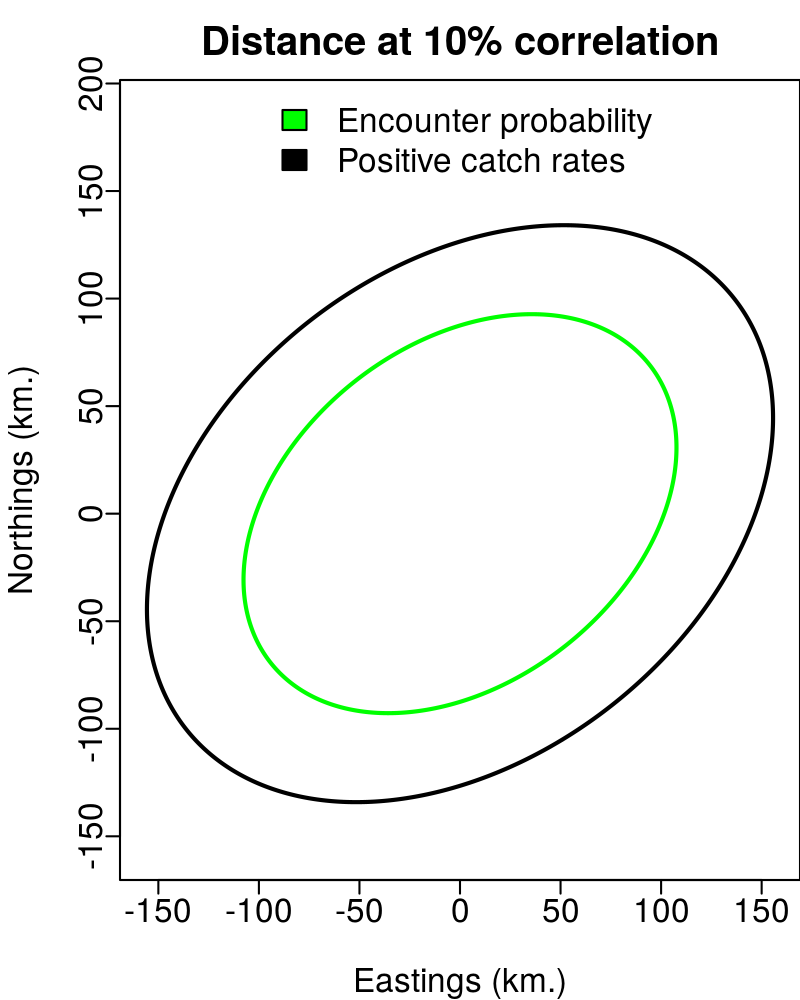
\includegraphics[width	=0.5\linewidth]{../../results/2017-04-08_M2/Aniso}
	\label{fig:Aniso}
	\caption{Anisotropic direction and strength}
\end{figure}

\begin{figure}[!ht]
	\center
	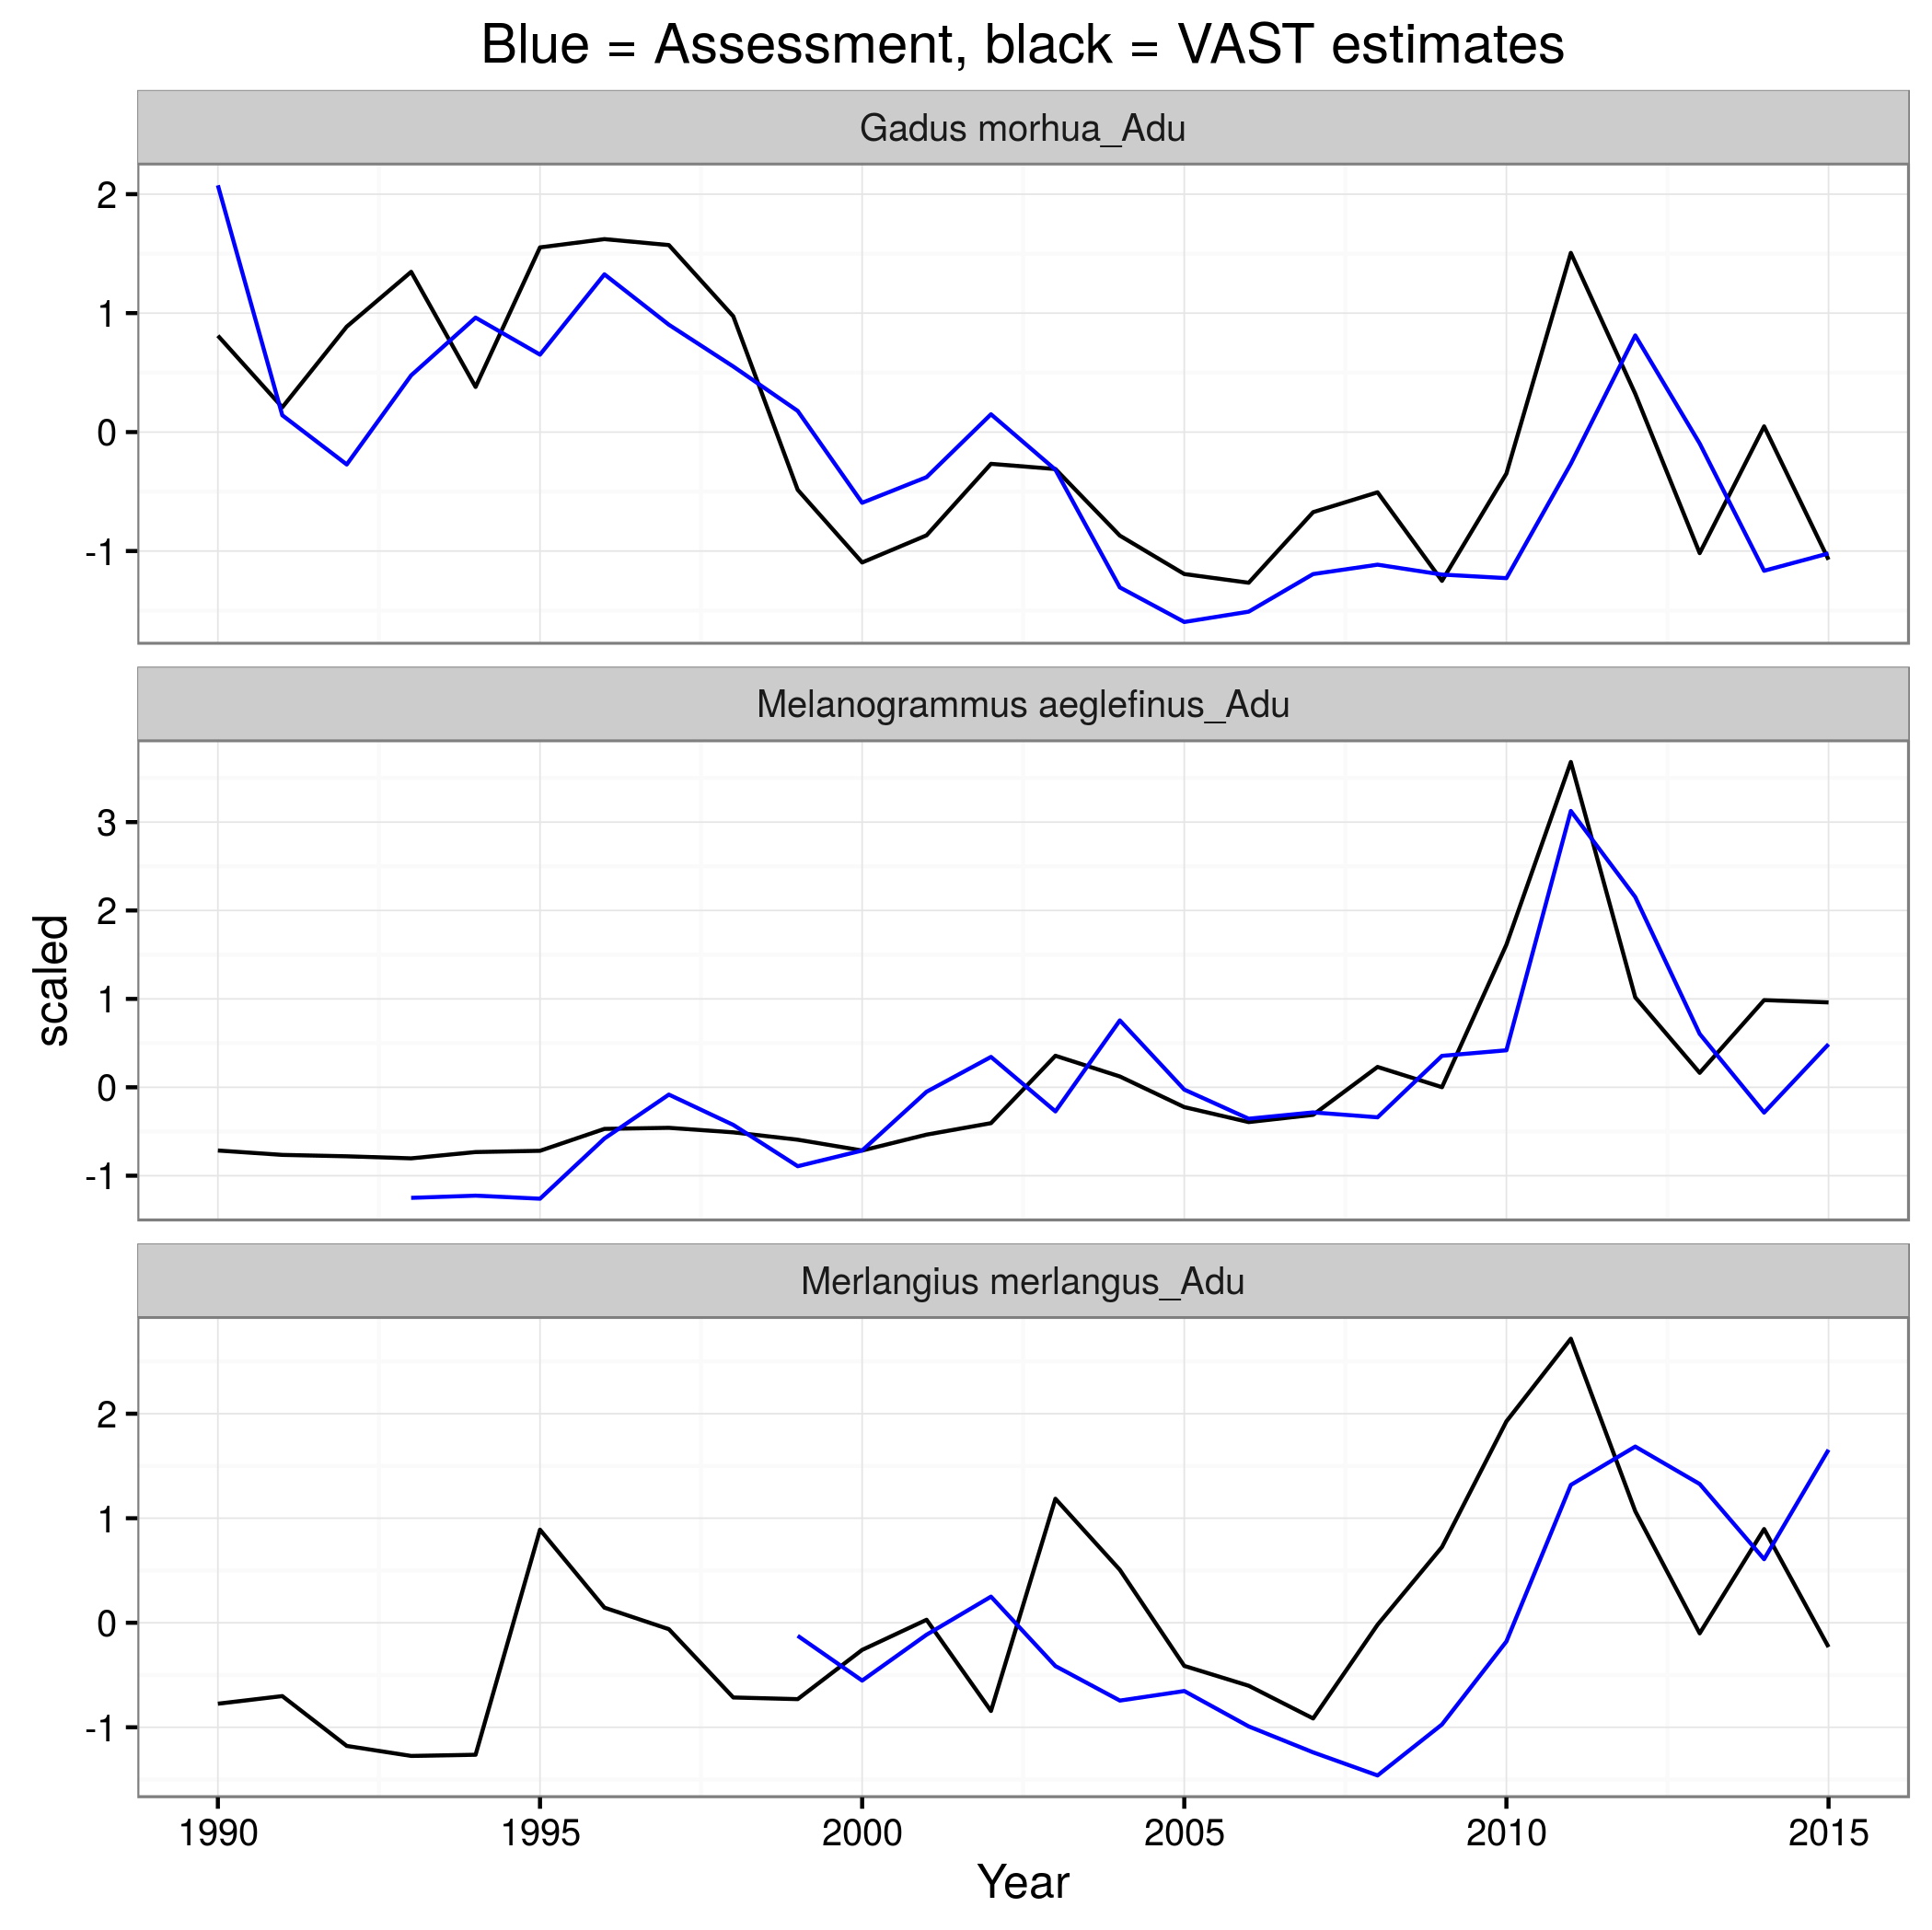
\includegraphics[width	=0.5\linewidth]{../../results/2017-04-08_M2/RealativeIndexVRelativeAssessSSB}
	\label{fig:IndexRel}
	\caption{Plot of relative index from VAST and relative assessment SSB
		for cod, haddock and whitinq}
\end{figure}

%%%%%%%%%%%%%%%%%%%%%%%%%%%%%%%%%%%%%%%%%%%%%%%%%%%%%%%%%%%%%%%%%%%%%%%%%%%%%%%%%%%%
\end{document}
